\documentclass[10pt]{article}

\def\Type{LessonCaelan}
\def\TypeNum{Lesson 8}
\def\TypeTitle{Chain Rule }
\def\Semester{Fall 2021} %Not Used 
\def\Course{MATH 1190 \& 1210}
\def\Targets{ {\bf\color{ForestGreen}D2} }

\usepackage{preambleDJ}




%%%%%%%%%%%% BEGIN DOCUMENT %%%%%%%%%%%%%%%
%%%%%%%%%%%% BEGIN DOCUMENT %%%%%%%%%%%%%%%
%%%%%%%%%%%% BEGIN DOCUMENT %%%%%%%%%%%%%%%
%%%%%%%%%%%% BEGIN DOCUMENT %%%%%%%%%%%%%%%
%%%%%%%%%%%% BEGIN DOCUMENT %%%%%%%%%%%%%%%



\begin{document}

\pagestyle{otherpages}
\thispagestyle{firstpage}
\vs{.4}

\textbf{Intended Learning Outcomes}
After this lesson, you will be able to 

\begin{itemize}
    \item Apply the chain rule to take the derivative. (\target{D2})
    \item Determine the order of applying differentiation rules when multiple rules are to be applied. (\target{D2})
\end{itemize}

\vspace{-0.5cm}

\hrulefill

{\bf \blue{Outer \& Inner Functions}}\\
{\bf\color{blue}Warm-up Exercise 1.} Suppose $h(x) = x^{\frac{3}{2}}$ and $j(x) = x^2 - x+1$.

\enumA{
    \item Define $(h\circ j)(x) = h(j(x))$. Note that $(h\circ j)(x)$ is a \textit{composite function}, where $h$ is the ``outside'' or ``outer'' function and $j$ is the ``inside'' or ``inner'' function. Write a formula for $(h\circ j)(x)$.
    
    \vfill

    
    \item  Define $(j\circ h)(x) = j(h(x))$.  Now $(j \circ h)$ is also a \textit{composite function}. This time, $j$ is the ``outside'' or ``outer'' function and $h$ is the ``inside'' or ``inner'' function. Write a formula for $(j\circ h)(x)$.
    
    \vfill

}

{\bf\color{blue}Warm-up Exercise 2.} The following are compositions of functions. Decide what the outer function $f$ and inner function $g$ are, testing your choices by finding $(f\circ g)(x)=f(g(x))$ in the space provided.\\

\enumA{
\item  \begin{tabular}{p{1.25in}ll}  $(x^2+2x-1)^4$ & {\large outer $f(x)=$\unline{1}{}{.25}} &\qquad {\large inner $g(x)=$\unline{1}{}{.25}} \\   \end{tabular}
\vs{.75}
\item   \begin{tabular}{p{1.25in}ll} $\sqrt{e^x+1}$ \qquad & {\large outer $f(x)=$\unline{1}{}{.25}} &\qquad {\large inner $g(x)=$\unline{1}{}{.25}} \\   \end{tabular}
\vs{.75}
\item  \begin{tabular}{p{1.25in}ll} $e^{\sqrt{x}}+1$  & {\large outer $f(x)=$\unline{1}{}{.25}} &\qquad {\large inner $g(x)=$\unline{1}{}{.25}} \\   \end{tabular}
\vs{.75}
}
%\item $(x^2+2x-1)^4$ \,\hfill 
%    {\large outer $f(x)=$\unline{1}{}{.25}}
%   \hfill
%    {\large inner $g(x)=$\unline{1}{}{.25}}
   % \\[0.75in]
%}

%\item $\sqrt{e^x+1}$ \,\hfill 
%    {\large outer $f(x)=$\unline{1}{}{.25}}
%\hfill
%    {\large inner $g(x)=$\unline{1}{}{.25}}
%    \\[0.75in]
%    
%
%\item $e^{\sqrt{x}}+1$ \,\hfill 
%    {\large outer $f(x)=$\unline{1}{}{.25}}
%   \hfill
%    {\large inner $g(x)=$\unline{1}{}{.25}}
%    \\[0.75in]



%\end{document} %end document here for pre-class assignment

%%%%%%%%%
\newpage%
%%%%%%%%%


{\bf \blue{ Chain Rule: Prime Notation or Lagrange Notation}}

The {\bf Chain Rule} gives a way to compute derivatives of compositions of functions. \\
{\em Key Idea:}\vs{.5}

{\bf Prime notation:} If $g$ is differentiable at $x$ and $f$ is differentiable at $g(x)$, then the composite function $f \circ g$ defined by $(f \circ g)(x)=f(g(x))$ is differentiable at $x$ and $(f \circ g)'$ is given by the formula \\\\

\hs{.5}$\ds \dfrac{d}{dx}\left[ (f\circ g)(x)\right]=$% \unline{1.8}{}{.25}$\\\\
\\\\

\

{\bf\color{blue} GOAL:} The following 2 exercises build skills needed in learning target {\bf\color{ForestGreen}D2}, an important learning target in MATH 1190 \& 1210. {\bf\color{ForestGreen}D2} prompts typically involve functions represented algebraically, graphically, or tabularly, and using all three of the product, quotient, and chain rules.

\

{\exercise{\color{ForestGreen}D2}} Use the derivative rules on the previous page to find the following derivatives:

\begin{enumerate}

\item[(a)]$\displaystyle\frac{d}{dx}\left[ (x^2+2x-1)^4 \right]$

\vfill

\item[(b)] $\displaystyle\frac{d}{dx}\left[ \sqrt{e^x+1} \right]$

\vfill

\item[(c)] $\displaystyle\frac{d}{dx}\left[ e^{\sqrt{x}}+1 \right]$

\vfill

\end{enumerate}


%%%%%%%%%
\newpage%
%%%%%%%%%


\exercise{\color{ForestGreen}D2} Find the following derivatives:

\begin{enumerate}
\item[(a)] $\displaystyle\frac{d}{dy}\left[ (y^2-1)^{3/2} \right]$

\vfill

\item[(b)] $\displaystyle\frac{d}{dy}\left[ y(y^2-1)^{3/2} \right]$

\vfill
\vfill

\item[(c)] $\displaystyle\frac{d}{dy}\left[ \frac{y(y^2-1)^{3/2}}{5y+1} \right]$

\vfill
\vfill
\vfill
\end{enumerate}


%%%%%%%%%
\newpage%
%%%%%%%%%


{\bf \blue{ Chain Rule: Leibnitz Notation}}

The {\bf Chain Rule} gives a way to compute derivatives of compositions of functions. Please fill in the blanks in the statement of the Chain Rule {\it using Leibniz notation} below. \\

{\bf Leibniz notation:} If $y$ is a differentiable function of $u$ and $u$ is a differentiable function of $x$, then \\

\hs{.5}$\ds \frac{dy}{dx}=$
\\

\exercise{\color{ForestGreen}D2} Let $w$ represent the weight (in pounds) of an average infant. The weight of an infant can be regarded as a function of the height $h$ (in inches) of the infant, and height can further be regarded as a function of age $t$ (in months):
\[w=w(h(t))\]
\enumA{
\item What are the units of measurement of $\dfrac{dw}{dt}$,  $\dfrac{dh}{dt}$, and $\dfrac{dw}{dh}$?\\

{\Large \,\hfill $\dfrac{dw}{dt}:$\unline{1.5}{}{.4} \hfill $\dfrac{dh}{dt}:$\unline{1.5}{}{.4} \hfill $\dfrac{dw}{dh}:$\unline{1.5}{}{.4} \hfill\,}\\

\mpageT{.5}{.5}[\hs{.3}]{
\item Given $w=w(h(t))$, use Leibniz notation to write down the derivative of $w$ with respect to $t$. Your answer should involve $\dfrac{dw}{dt}$,  $\dfrac{dh}{dt}$, and $\dfrac{dw}{dh}$.
}{
\item Is $\dfrac{dw}{dh}$ positive, negative, or zero? Give a description of the relationship \& a mathematical justification incorporating the context of this problem while explaining your answer. ({\bf NOTE:} explanations are of the utmost importance in this class. We care more about your thought process than your final answer, so please make sure your answers are well-supported!)
}
}


%%%%%%%%%
\newpage%
%%%%%%%%%


\,

\vspace{-0.5in}

%
{\bf\color{blue}Extra Practice 1.}
%
\reversemarginpar\marginnote{\fbox{\bf\color{ForestGreen}D2}} 
%
Let $k(x)=f(g(x))$, where $f$ and $g$ are functions whose graphs are shown below. What is the value of $k'(5)$?  \\
\mpageT{.4}{.6}{
\begin{center}
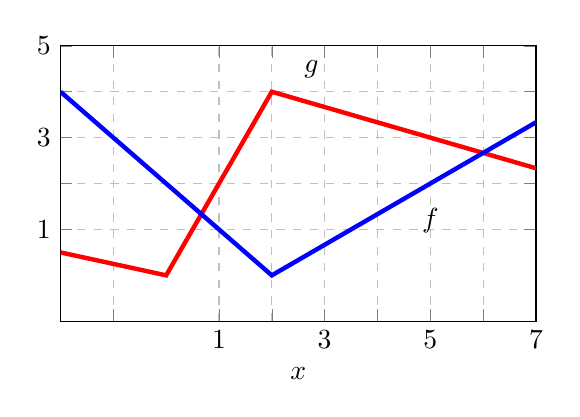
\begin{tikzpicture}
  \begin{axis}[
    xlabel={$x$},
    xtick       = {-2,-1,1,2,3,4,5,6,7},
    xticklabels = { , ,$1$, ,$3$ , ,$5$ , , $7$},
    ytick       = {-1,1,2,3,4,5},
    yticklabels = { ,$1$, ,$3$ , ,$5$ },
    samples     = 320,
    domain      = -3.5:3.5,
    %restrict y to domain=-2.5:4.5,
    xmin = -2, xmax = 7,
    ymin = -1, ymax = 5,
    width = 3in, height = 2in,
    grid=both, grid style=dashed
  ]
  \draw[red,ultra thick] (-2,0.5) -- (0,0) -- (2,4) -- (8,2);
  \node at (2.75,4.5) {$g$};
  \draw[blue,ultra thick] (-2,4) -- (2,0) -- (8,4);
  \node at (5,1.2) {$f$};
\end{axis}
\end{tikzpicture}
\end{center}
}{
\vs{2}
}

{\bf\color{blue}Extra Practice 2.}
%
\reversemarginpar\marginnote{\fbox{\bf\color{ForestGreen}D2}} 
%
Find the following derivative: $\dfrac{d}{dx}\left[\sqrt{\dfrac{1+x^2e^x}{1-e^x}} \right]$

\vfill

{\bf\color{blue}Extra Practice 3.}
%
\reversemarginpar\marginnote{\fbox{\bf\color{ForestGreen}D2}} 
%
The flux $F$ of blood through a vessel -- that is, the volume of blood per unit time that flows past a given point -- can be regarded as a function of the radius $R$ of the vessel. In particular, when $R$ changes, so too does $F$.

\begin{enumerate}
\item[(a)] Assuming $F$ is measured in $\dfrac{mm^3}{sec}$, $R$ is measured in $mm$, and $t$ is measured in $sec$, what are the units of the following derivatives?\\
\,
\hfill
{\large $\dfrac{dF}{dt}$:\unline{1.25}{}{.4}}
\hfill
{\large $\dfrac{dF}{dR}$: \unline{1.25}{}{.4}}
\hfill
{\large $\dfrac{dR}{dt}$: \unline{1.25}{}{.4}}
\hfill
\,\\[0.2in]

\item[(b)] When the human body experiences a drop in blood pressure -- due to, for example, blood loss or dehydration -- it creates and distributes a hormone called angiotensin to raise blood pressure by decreasing blood vessels' radii. How are $\dfrac{dF}{dt}$ and $\dfrac{dF}{dR}$ related once angiotensin has been created and distributed?\\

\begin{enumerate}
\item[A.] They are the same.
\item[B.] Both are positive.
\item[C.] Both are negative.
\item[D.] One is positive and one is negative.
\item[E.] none of the other answers\\
\end{enumerate}



\end{enumerate}


\end{document}
